%% muKV, 10-page version (2026-09-07). Built from PAPER_HOTMOBILE_2027.tex (source of truth for
%% every number). Structure: intro, background, design, control, implementation, evaluation,
%% related work, conclusion. No em dashes; captions under 35 words; table captions above.
\documentclass[sigconf, anonymous=false, screen=true]{acmart}
\settopmatter{printacmref=false}
\renewcommand\footnotetextcopyrightpermission[1]{}
\pagestyle{plain}
\acmConference[HotMobile '27]{International Workshop on Mobile Computing Systems and Applications}{2027}{}
\usepackage{booktabs}
\usepackage{multirow}
\newcommand{\yes}{$\bullet$}
\newcommand{\no}{$\cdot$}
\usepackage{xcolor}
\usepackage{hyperref}
\usepackage{microtype}
\usepackage{graphicx}
\graphicspath{{figures/}}
\usepackage{enumitem}
\newcommand{\slb}{/\allowbreak}
\newcommand{\ub}{\_\allowbreak}
\setlength{\emergencystretch}{2em}
\definecolor{kvgreen}{RGB}{40, 174, 96}
\definecolor{kvred}{RGB}{192, 57, 43}
\definecolor{kvgray}{RGB}{85, 85, 85}
\newcommand{\good}[1]{\textcolor{kvgreen}{\textbf{#1}}}
\newcommand{\bad}[1]{\textcolor{kvred}{\textbf{#1}}}
\newcommand{\muKV}{$\mu$KV}
\newcommand{\C}{\,\textdegree C}

\begin{document}

\title[\muKV: Energy- and Thermal-Aware KV Eviction on a Phone]{\muKV: Energy- and Thermal-Aware KV-Cache Eviction for LLM Inference on a Phone}

\author{Md Romyull Islam}
\affiliation{%
  \institution{Kennesaw State University}
  \city{Marietta}
  \state{Georgia}
  \country{USA}
}
\email{romyullislam2012@gmail.com}

\begin{abstract}
On a phone the KV cache, not compute, limits sustained LLM decode. The policies that bound it were built for server GPUs. Three properties of a real on-device engine break them. One cell array serves every head and layer, so a cell is freed only when every head and every layer drops it. SnapKV reports an 8.2 times smaller cache; on this engine it retains 68\% of the cells at a matched budget and 94\% at its own. Reading attention scores forces the FlashAttention-off path, so score-reading evictors decode at 0.12 to 0.30 times the full cache on the phone GPU. Compaction through the state API needs a second full context, and the OS kills Phi-3-mini at 16K. \muKV\ respects all three. It scores tokens inside the FlashAttention prefill graph through a small side node. It selects one keep set for all heads and layers. It compacts in place, so peak memory never rises. Two controllers sit beside the cache. A reduce-only clock watchdog with CPU and GPU ladders keeps the vendor throttle unreachable. A per-request scheduler picks the GPU clock plan, the cache budget and the answer cap from the battery state, and two loops correct it. On a OnePlus 15, \muKV\ decodes 4.8 times faster than the full cache on the CPU and 1.23 times on the Adreno GPU, at 7\% of the cells and 62\% less energy. It ties the full cache on 392 retrieval cells and stays within 0.1 to 3.7 F1 on LongBench at 13\% of the cache. With 1-bit weights it finishes a workload that deep-throttles the full cache. Through a real discharge from 91 to 11\%, its two lower tiers cut energy per request by 15\% and 43\%.
\end{abstract}

\keywords{Mobile LLM inference, KV cache eviction, FlashAttention, thermal management, energy-aware scheduling, on-device AI}

\maketitle
\makeatletter\fancyhead[RO]{\@headfootfont HotMobile '27}\fancyhead[LE]{\@headfootfont HotMobile '27}\makeatother

\section{Introduction}
\label{sec:intro}

Small instruction-tuned models now run interactively on flagship phones. For a sustained generation the wall is the KV cache, not the matrix multiply. Every decode step reads the whole cache once per layer. Past a thousand tokens the step is bound by DRAM bandwidth. The DRAM heats, the vendor thermal engine cuts the clock, and the battery drains. Cache size sets traffic, traffic sets power, power sets temperature, temperature sets the throttle, and the throttle sets throughput. A mobile cache policy must therefore be judged on quality, throughput, heat and energy together, on real hardware.

The policies that bound the cache were built for server GPUs and judged by perplexity alone: H2O~\cite{zhang2023h2o}, TOVA~\cite{oren2024tova}, SnapKV~\cite{li2024snapkv}, StreamingLLM~\cite{xiao2024streamingllm} and Ada-KV~\cite{feng2025adakv}. We ran each in its published configuration on a OnePlus 15 inside \texttt{llama.cpp}. Three properties of the engine broke them.

\begin{itemize}[leftmargin=*, itemsep=1pt]
\item \textbf{Budgets do not materialize.} The engine keeps one cell array shared by every head and layer. A cell is freed only when every head and every layer drops it. SnapKV selects per head and reports an 8.2 times smaller cache at 16K inputs~\cite{li2024snapkv}. At a matched budget of 1024 per head on this engine it keeps 68\% of the cells on Llama-3.2-1B and 85\% on Phi-3-mini. At its own budget of 2048 per head it keeps 94\%. H2O reports a 5 to 10 times smaller cache at a 20\% budget~\cite{zhang2023h2o}; at that budget here it keeps 92 to 99.8\%.
\item \textbf{Scores cost the fast path.} A policy that reads post-softmax attention cannot use the fused FlashAttention kernel. Every score-reading evictor decodes at 0.12 to 0.30 times the full cache on the phone GPU. Evicting makes it slower.
\item \textbf{Compaction doubles memory.} The state API restores survivors into a second context. Phi-3-mini at 16K needs two 6.4\,GB caches plus 2.4\,GB of weights, and the OS kills it. The same call fails on a 24\,GB desktop GPU.
\end{itemize}

\muKV\ is an evictor designed around these facts, with the two controllers a phone needs beside it (Figure~\ref{fig:architecture}). It computes selection scores inside the FlashAttention prefill graph through a small side node. It selects one keep set of $K$ cells for all heads and layers, so eviction frees cells. It compacts in place: survivors slide into a dense prefix inside the tensors prefill already allocated. A reduce-only watchdog steps the CPU and GPU clocks down along temperature ladders anchored at the measured vendor triggers. A per-request scheduler picks the GPU clock plan, the cache budget and the answer cap from the battery state. It predicts the request's cost from a measured table, and two loops correct its lever when time or energy misses.

We evaluate on a OnePlus 15 (Snapdragon 8 Elite Gen 5, Adreno 840) with four models and nine policies. Quality is perplexity on a slice disjoint from the prompt, retrieval on 392 needle cells, and LongBench F1. Cost is prefill and decode time, live cells, peak resident set, DDR and skin temperature, and system energy, all under a cooling gate. This paper makes five contributions.

\begin{enumerate}[label=(\roman*), leftmargin=*, itemsep=1pt]
\item The realizability gap: nominal per-head budgets do not compact on a sequence-level engine, measured for five policies on four models (\S\ref{sec:eval-cpu}, \S\ref{sec:eval-gpu}).
\item In-graph scoring, one keep set and in-place compaction, which keep an attention-driven evictor on the FlashAttention path and make an infeasible configuration run (\S\ref{sec:design}).
\item A thermal watchdog with CPU and GPU ladders anchored at the measured vendor trigger, and the negative result that cache size does not cap peak temperature (\S\ref{sec:control}, \S\ref{sec:eval-thermal}).
\item An energy-aware scheduler with one lever and two loops, measured through a real battery discharge and under provoked disturbances (\S\ref{sec:eval-energy}).
\item A multi-axis on-device evaluation with every baseline in its own published configuration (\S\ref{sec:eval}).
\end{enumerate}

\section{Background and Motivation}
\label{sec:bg}

\paragraph{Decode is bandwidth-bound.} Autoregressive decode reads all cached keys and values every step. Phi-3-mini at a 2K context holds about 1.2\,GiB of f16 KV and reads roughly 750\,MB per attention pass. On LPDDR5X at about 50\,GB/s this dominates the step. The cache also sets heat. Across our 372-cell on-device dataset, live cache correlates with DDR temperature at $r{=}0.80$ and with throughput at $r{=}{-}0.77$.

\paragraph{Eviction policies.} H2O~\cite{zhang2023h2o} keeps heavy hitters by accumulated attention plus recent tokens, split evenly, and reads attention every step; it reports a 5 to 10 times smaller cache at a 20\% budget. TOVA~\cite{oren2024tova} drops the position with the least attention from the last query, averaged over the heads of a layer, and reports full-model quality at one eighth of the cache with 4.8 times the throughput. SnapKV~\cite{li2024snapkv} freezes a per-head top-$K$ at the end of prefill from an observation window and reports 3.6 times faster decode and an 8.2 times smaller cache at 16K inputs. StreamingLLM~\cite{xiao2024streamingllm} keeps 4 sink tokens and a sliding window with no scores; it reports 22.2 times the speed of window recomputation and states that it adds no long-term memory. Ada-KV~\cite{feng2025adakv} allocates one layer budget across heads from a global top-$B$ with a safeguard of 0.2, and needs FlashAttention-2's variable-length kernel~\cite{dao2023flashattention2} plus a custom CUDA kernel, both absent on the mobile stack. KIVI~\cite{liu2024kivi} quantizes instead of evicting. KVzip~\cite{kim2025kvzip} scores by reconstruction. Both are orthogonal.

\paragraph{The architectural conflict.} FlashAttention~\cite{dao2022flashattention} fuses softmax into the kernel and never writes the attention tensor to memory. A policy that reads attention scores cannot use the fused kernel and is locked to the slow path. On the phone this, not retention, decides speed. StreamingLLM retains about as few cells as \muKV\ yet pays the slow path in the CPU runs. Every per-head evictor pays it everywhere.

\paragraph{The engine.} \texttt{llama.cpp}~\cite{llamacpp}, like every on-device engine we know of, stores the cache as one array of cells indexed by position and shared across heads and layers. Its cache API removes positions, so a per-head keep set can only be realized as the union over heads. Compaction goes through the state API, which serializes the cache and restores it into a second context. Neither fact is visible on a server with per-head paged storage. Both decide what a policy can do on a phone.

\paragraph{Thermal and energy control on phones.} zTT~\cite{kim2021ztt} and FUSE~\cite{liu2022fuse} act on CPU and GPU frequency from temperature or phase, with no cache signal. The vendor engine on our SoC deep-throttles the prime cores to 883\,MHz the moment the battery reaches 50\C. It caps the GPU at 726\,MHz when DDR passes 64\C. No shipped phone changes an LLM's clock, context or answer length by battery state. EnerInfer~\cite{zou2026enerinfer} is the closest research system and excludes battery level by design. Kim, Imes and Hoffmann~\cite{kim2015racepace} prove that an energy-optimal schedule under a deadline uses at most two configurations. JouleGuard~\cite{hoffmann2015jouleguard} couples an accuracy loop and an energy loop through model error. \muKV's scheduler applies both results.

\begin{figure*}[tp]
\centering
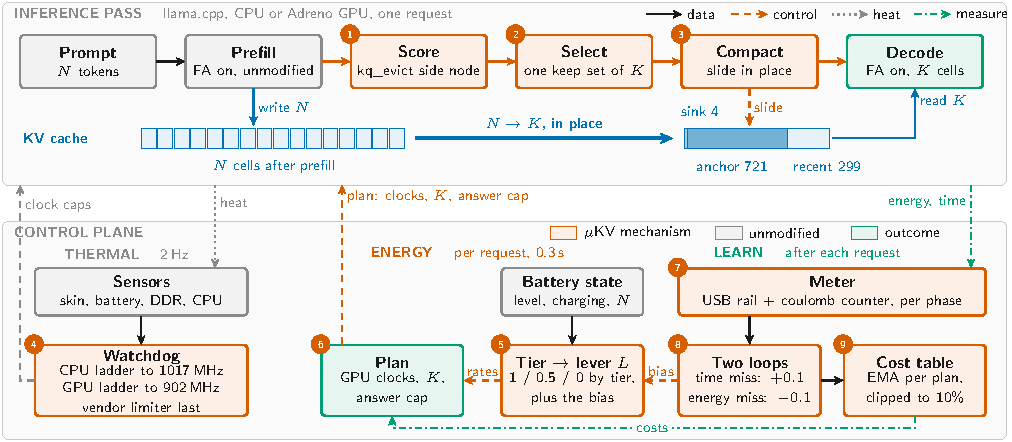
\includegraphics[width=0.96\textwidth]{fig_architecture_tikz.pdf}
\caption{\muKV\ on the phone. Top: the inference pass, with scoring, selection and compaction (1 to 3) as the only changes. Bottom: the thermal, energy and learning columns of the control plane (4 to 9).}
\label{fig:architecture}
\end{figure*}

\section{\muKV\ Design}
\label{sec:design}

Figure~\ref{fig:architecture} shows the system. The inference pass is unmodified \texttt{llama.cpp} with three insertions between prefill and decode: score, select, compact. Figure~\ref{fig:mechanism} shows where the scores come from, how one keep set is chosen, and why it compacts while per-head keep sets cannot.

\begin{figure}[tb]
\centering
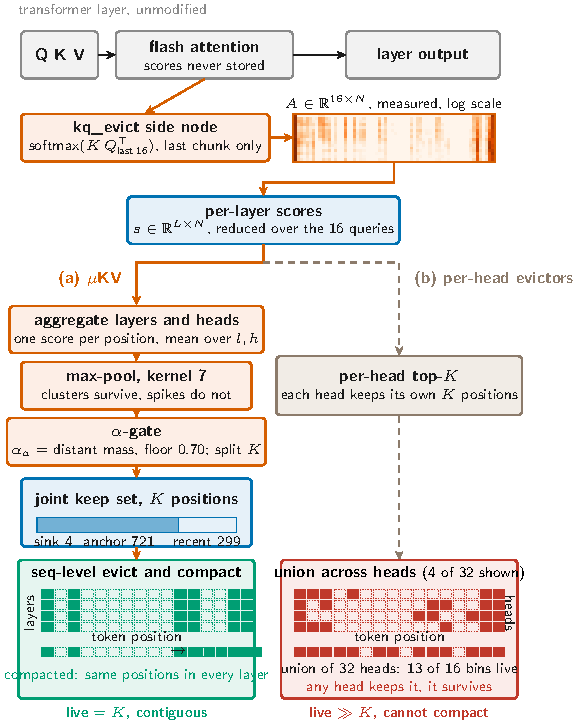
\includegraphics[width=0.92\columnwidth]{fig_mechanism_tikz.pdf}
\caption{Scores, selection and the two outcomes. Heatmap and keep sets are measured on Llama-3.2-1B, layer 8, 16 position bins: the union over 32 heads keeps 13 bins, the joint set 6.}
\label{fig:mechanism}
\end{figure}

\subsection{Scoring inside the FlashAttention graph}
\label{sec:design-score}

The selection below needs post-softmax attention, which the fused kernel never materializes. \muKV\ adds a small \texttt{kq\_evict} side node to the prefill graph instead of leaving the fast path. The node computes $\mathrm{softmax}(K Q^{\top})$ for the last 16 queries of the last prefill chunk only, since earlier chunks' scores are overwritten anyway. It reduces over queries to one score per layer, head and position, $\bar A_{l,h,p}$. The node is a graph output, so the mid-graph interception that corrupts this Vulkan backend cannot touch it. It costs 1.2\% of prefill on the CPU (paired, $n{=}29$) and 138 against 131\,s on the GPU. Selection is bit-identical to a FlashAttention-off capture, verified by teacher-forced perplexity.

\subsection{One keep set for all heads and layers}
\label{sec:design-select}

Selection is sequence-level. It reduces $\bar A_{l,h,p}$ to one score per position and keeps one set of $K$ positions for every head and layer, which is what lets the cache compact. No step needs a forward pass.

\paragraph{One score per position.} The position score is the mean of $\bar A_{l,h,p}$ over layers and heads. A 7-position max-pool then replaces each score by the largest in its neighbourhood, SnapKV's clustering step~\cite{li2024snapkv}, so a run of related tokens survives together instead of one spike.

\paragraph{Per-prompt split.} The fraction of attention mass outside the recent window, $\alpha_a$, sets how many of the $K$ cells are distant anchors: $n_\mathrm{anchor} = \mathrm{round}(\alpha_a (K - n_\mathrm{sink}))$, with $\alpha_a$ floored at 0.70 and capped at 0.95. The rest is the recent window. Retrieval prompts, whose mass sits in the prompt, get more anchors; chat prompts get more window. On the 9737-token prompt $\alpha_a = 0.71$, so $K{=}1024$ is 4 sinks, 721 anchors and 299 recent cells.

\paragraph{Keep set.} The top $n_\mathrm{anchor}$ positions by pooled score survive as anchors, plus four sink tokens~\cite{xiao2024streamingllm}. Everything else in the prompt is evicted. During decode the keep set stays frozen while the recent window slides.

\paragraph{A per-head gate, removed.} Earlier versions sized a per-head budget from each head's peak attention through a closed-form ramp, $K_h = \mathrm{round}(K\,\mu(m_h))$ with $\mu\in[0.7,1.3]$, and unioned the per-head top-$K_h$ sets into a candidate pool ahead of the steps above. Measured on every cell, that pool holds 96.5 to 99.8\% of the prompt at $K{=}1024$. The union of 32 per-head sets is the whole prompt, the same effect that stops per-head evictors from compacting. We verified the removal on the 9737-token prompt: with the gate bypassed the keep set is identical, 721 of 721 positions, and so is the generated text. Every cell in this paper ran with the gate in place, which changes nothing; the released configuration bypasses it.

\paragraph{Sizing $K$.} Prompt length under-determines the budget. A short instruction that produces a long answer needs a cache that grows with the output. A long prompt with a short answer needs only a slice. In a controlled retention test on Llama-3.2-1B, the smallest $K$ that still retrieves a fact placed before a span of generated text scales with the span: 256 cells at 64 tokens, 4096 at 2048. The prompt was fixed at 36 tokens. \muKV\ therefore sizes $K$ from the request's demand, the larger of a retrieval floor and a generation floor, clipped to a thermal admission cap. The tables below use the nominal $K{=}1024$.

\subsection{In-place compaction and decode}
\label{sec:design-compact}

Compaction through the state API restores survivors into a second context. Peak cache memory doubles at that instant. On unified memory that is fatal: Phi-3-mini at 16K needs $2\times6144$\,MiB plus 2.4\,GB of weights, and Android killed the process and six co-resident apps, twice. \texttt{endurkv\_compact\_seq()} instead slides survivors into a dense prefix in bounded chunks inside the tensors prefill already allocated. Peak memory does not rise, and the same configuration runs at 874 cells. The two modes produce identical keep sets; across four model families and a 64K sweep their perplexities agree to 0.15\%. An earlier variant ran prefill FA-off and swapped the compacted cache into an FA-on context. It selects the same cells at 10 to 15\% more prefill time and appears in the CPU table as \muKV\ (state-swap).

Decode runs over the $K$-cell cache with the fused kernel. The keep set stays frozen while the recent window slides. A re-eviction fires only when the live cache exceeds $1.25\times(n_\mathrm{anchor}+n_\mathrm{recent})$, which bounds the decode-mean cache near 2K cells on a 4K generation. On the CPU the K half of the cache is stored as q8\_0, which halves K-side bytes and pays only above about a 1\,GB cache. On the GPU every policy runs f16, because quantized KV is numerically broken on this Adreno driver.

\section{Thermal and Energy Control}
\label{sec:control}

\subsection{Reduce-only clock watchdog}
\label{sec:watchdog}

A userspace daemon samples skin, battery, DDR and CPU temperature at 2\,Hz. It lowers a clock cap one step at a time and never raises it above base. Its ladders are anchored at measured vendor triggers, not chosen in theory. On the CPU the vendor deep-throttles both clusters to 883\,MHz the instant the battery reaches 50\C\ (\S\ref{sec:eval-thermal}). The ladder therefore maps battery 47.0\slb 48.0\slb 48.5\slb 49.0\slb 49.5\C\ and skin 50.0\slb 51.0\slb 51.5\slb 52.0\slb 52.5\C\ to caps of 1497\slb 1382\slb 1267\slb 1132\slb 1017\,MHz. The floor stays above the cliff, so the watchdog never self-throttles. On the GPU the vendor limiter drops to 726\,MHz when DDR passes about 64\C. A second ladder writes 1050, 967 and 902\,MHz at DDR 60, 62 and 63.5\C, with 1.5\C\ hysteresis. The kernel applies the lower of the user cap and the vendor cap, so the ladders act earlier than the vendor and never later. On a cold phone both stay dormant. The watchdog acts on the clock only; \S\ref{sec:eval-thermal} shows that a cache budget tied to temperature does not cap peak heat.

\subsection{Energy-aware scheduling: one lever, two loops}
\label{sec:sched}

\begin{figure*}[tp]
\centering

\includegraphics[width=0.96\textwidth]{fig_control_plane_tikz.pdf}
\caption{The energy-aware control plane, once per request: sense, decide, act, run, measure, learn. The thermal guard acts on the clock beside it.}
\label{fig:controlplane}
\end{figure*}

The scheduler runs once per request in about 0.3\,s (Figure~\ref{fig:controlplane}). It reads the battery level, the charging state, the prompt length, and whether the caller fixed an answer length. A tier follows: mains or above 50\%, 21 to 50\%, and 20\% or below. The tier sets a lever $L\in\{1, 0.5, 0\}$ plus a learned bias. $L$ fixes every rate the scheduler trades at. The exchange rate a step must beat is 1.5, 0.8 or 0.5\,J saved per second given up. A quality floor and a time slack follow it. So does the answer cap when the caller left the length open: 4096, 1024 or 512 tokens.

\paragraph{Plan.} A measured cost table holds energy and time per plan. A plan is a GPU clock cap for prefill, one for decode, and the cache budget. The walk down the plan ladder takes a step only if the predicted saving beats the exchange rate and the predicted time stays inside the budget. The split plan, prefill at 1200\,MHz and decode at 902, is the two-configuration schedule of Kim, Imes and Hoffmann~\cite{kim2015racepace}. It is also the best measured point by energy-delay product (\S\ref{sec:eval-energy}).

\paragraph{Two loops on model error.} After the request the meter reports energy and time per phase. If time ran more than 5\% over the budget the plan was chosen under, the performance loop moves the bias 0.1 toward performance. If energy ran more than 5\% over its prediction, the energy loop moves it 0.1 toward energy. When both are met the bias decays by 0.05 toward the tier default. The bias is clamped to $\pm0.3$. This is the JouleGuard coupling~\cite{hoffmann2015jouleguard}: the loops act on the model's error, so a disturbance moves the lever and a quiet request moves it back. Knobs only one loop feels belong to that loop: the decode clock and the answer cap to the energy loop, the CPU clock to the watchdog. Only the prefill clock is shared, and the lever arbitrates it. The cost table learns by an exponential moving average clipped to 10\% per request, so interference cannot pass for a plan's cost. There is no online policy learning on the user's phone. The decision is a table walk, the table is seeded from measurements, and the loops correct it. A contextual bandit trained on 24 real requests chose the rule's plan in 13 of 15 free choices; the other two were the low tier's 726\,MHz arm, which tied within 0.002. Its learning cost 15.7\,kJ and 149 minutes of phone time, which the rule does not pay.

\section{Implementation}
\label{sec:impl}

\muKV\ is a \texttt{llama.cpp} extension we call \texttt{eviction\ub bench}: a 4.2K-line driver plus engine patches. The patches add the \texttt{kq\_evict} side node on the CPU and Vulkan backends, the score reduction and split, \texttt{endurkv\_compact\_seq()}, and a cell-index removal call for multimodal caches. The driver also carries faithful ports of SnapKV, Ada-KV, H2O, TOVA and StreamingLLM in their published configurations. The watchdog and the scheduler are shell daemons on the phone. The cost table is a text file, and a decision is a table walk. Sensors are read from sysfs at 2 to 5\,Hz. Energy integrates the USB rail ($V{\cdot}I$) and the battery coulomb counter, split at the prefill and decode boundary, with charging disabled during every timed cell. The GPU cap writes both the kgsl power-level index and the clock, because the vendor engine clears a plain clock cap mid-request.

\section{Evaluation}
\label{sec:eval}

\paragraph{Setup.} OnePlus 15: Snapdragon 8 Elite Gen 5, 16\,GB unified memory, Adreno 840. Models: Llama-3.2-1B, Phi-3-mini-128k and gemma-2-2b-it in Q4\ub K\ub M, and PrismML's 1-bit Bonsai-8B~\cite{prismml2026bonsai}. Every timed cell starts behind a cooling gate (DDR $\le 35\C$, battery $\le 33\C$) with charging off, on one build, under the vendor's own DVFS and thermal engine. The vendor's clock cap is the same for every policy. Baselines run their own papers' selection rules. The tables use a matched budget of 1024. SnapKV and Ada-KV keep 1024 cells per head (window 64, kernel 5; Ada-KV safeguard 0.2). H2O keeps 1024 per head, split evenly between heavy hitters and recent tokens. TOVA keeps 1024 per layer with 4 sinks. StreamingLLM keeps 4 sinks and 1020 recent cells. A second campaign runs every baseline at its own published budget (\S\ref{sec:eval-cpu}). An RTX 4500 Ada and a Jetson Orin NX serve LongBench and the disjoint-slice perplexity, which needs a second context beside the prompt. \muKV\ runs with $K{=}1024$ and the watchdog throughout.

\subsection{Sustained decode on the CPU}
\label{sec:eval-cpu}

\begin{table*}[tp]
\caption{Sustained decode on the CPU, cold start, charging off. Upper two blocks: 9737-token prompt, 4096 generated, every policy at $K{=}1024$. Lower two: the same text (7542 and 6382 tokens), 2048 generated, baselines at their published budgets. Live cells: after prefill (\muKV\ decode mean in parentheses).}
\label{tab:cpu}
\centering\footnotesize
\setlength{\tabcolsep}{4pt}
\begin{tabular}{l l l r r r r r r r}
\toprule
\textbf{Model} & \textbf{Policy} & \textbf{Budget} & \textbf{tok/s} & \textbf{Prefill (s)} & \textbf{Wall (s)} & \textbf{Live cells} & \textbf{RSS (MB)} & \textbf{DDR (\textdegree C)} & \textbf{Energy (mWh)} \\
\midrule
\multirow{8}{*}{Llama-3.2-1B}
 & vanilla (full cache) & 1024 & 5.0 & 229 & 1055 & 9737 & 2102 & 59.8 & 1033 \\
 & \textbf{\muKV} & 1024 & \good{24.2} & \good{226} & \good{406} & 721 (1980) & 2154 & \good{54.4} & \good{391} \\
 & \muKV\ (state-swap) & 1024 & 22.7 & 250 & 438 & 733 (1984) & 2235 & 58.3 & 546 \\
 & SnapKV & 1024 & 6.8 & 287 & 902 & 5929 & 2236 & 56.3 & 818 \\
 & Ada-KV & 1024 & 6.7 & 252 & 875 & 3484 & 2236 & 57.1 & 1002 \\
 & StreamingLLM & 1024 & 6.6 & 250 & 877 & 777 & 2236 & 56.7 & 1052 \\
 & H2O & 1024 & 5.8 & 292 & 1006 & 6110 & 2312 & 54.8 & 1094 \\
 & TOVA & 1024 & 6.0 & 253 & 947 & 4091 & 2235 & 54.4 & 1069 \\
\midrule
\multirow{7}{*}{Bonsai-8B (1-bit)}
 & vanilla (full cache) & 1024 & 1.0 & 1058 & 5137 & 10074 & 4393 & \bad{72.2} & 5758 \\
 & \textbf{\muKV} & 1024 & \good{4.5} & 1073 & \good{2012} & 789 (1993) & 4517 & \good{62.5} & \good{2312} \\
 & SnapKV & 1024 & 1.1 & 1103 & 4713 & 10015 & 4475 & 67.9 & 5476 \\
 & Ada-KV & 1024 & 1.6 & 1191 & 3718 & 6514 & 4580 & 65.2 & 3971 \\
 & StreamingLLM & 1024 & 1.6 & 1161 & 3777 & 858 & 4580 & 63.7 & 4012 \\
 & H2O & 1024 & 1.5 & 1214 & 3900 & 9587 & 4748 & 63.3 & 4136 \\
 & TOVA & 1024 & 1.6 & 1149 & 3841 & 7116 & 4580 & 67.2 & 4581 \\
\midrule
\multirow{7}{*}{Phi-3-mini}
 & vanilla (full cache) & 1024 & 1.2 & 381 & 2063 & 7542 & 10679 & 60.6 & 2046 \\
 & \textbf{\muKV} & 1024 & \good{5.5} & 471 & \good{841} & 929 & 10764 & \good{56.3} & \good{926} \\
 & SnapKV & 1024/head & 1.7 & 759 & 1980 & 7130 & 10906 & 66.0 & 2530 \\
 & Ada-KV & 2048 & 1.7 & 702 & 1908 & 7086 & 10906 & 66.8 & 2479 \\
 & StreamingLLM & 4+2000 & 2.0 & 472 & 1493 & 2000 & 10680 & 57.1 & 1311 \\
 & H2O & 20\% & 1.7 & 1092 & 2305 & 7542 & 11018 & 62.5 & 2660 \\
 & TOVA & 2048 & 1.7 & 670 & 1856 & 6425 & 10645 & 62.9 & 2380 \\
\midrule
\multirow{7}{*}{gemma-2-2b-it}
 & vanilla (full cache) & 1024 & 3.9 & 206 & 735 & 6382 & 4971 & 58.7 & 974 \\
 & \textbf{\muKV} & 1024 & \good{9.3} & 206 & \good{427} & 804 & 4978 & \good{58.7} & \good{589} \\
 & SnapKV & 1024/head & 4.9 & 496 & 913 & 6297 & 5040 & 60.6 & 1005 \\
 & Ada-KV & 2048 & 5.0 & 500 & 909 & 6222 & 5040 & 60.6 & 989 \\
 & StreamingLLM & 4+2000 & 4.9 & 234 & 654 & 2000 & 4971 & 57.9 & 751 \\
 & H2O & 20\% & 3.9 & 493 & 1017 & 6382 & 5118 & 56.0 & 1071 \\
 & TOVA & 2048 & 3.9 & 490 & 1022 & 6060 & 5040 & 56.0 & 1063 \\
\bottomrule
\end{tabular}
\end{table*}

Table~\ref{tab:cpu} runs a 9.7K-token prompt followed by 4096 generated tokens on the CPU. A cell sustains pressure for 7 to 85 minutes. Figure~\ref{fig:cache-trajectory} shows the mechanism. Every policy builds the full prompt cache during prefill. \muKV\ then compacts to 721 cells, and its decode-time re-eviction keeps the cache bounded near 2K. SnapKV can only drop to 5.9K cells, and vanilla grows without bound. On Llama-3.2-1B the bounded cache buys 24.2 against 5.0\,tok/s, 2.6 times less wall time and 62\% less energy. Its DDR peak is the coolest of any policy, 5\C\ below vanilla. Both policies run the same vendor-clamped 1.6\,GHz, so the heat comes from memory traffic, not the clock.

\begin{figure}[tb]
\centering
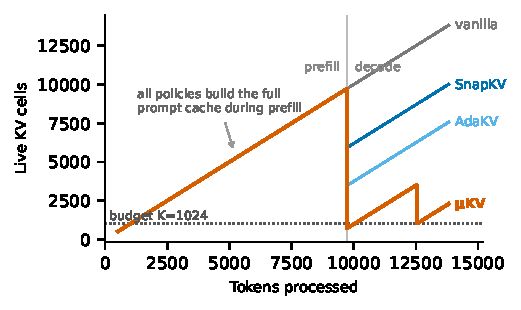
\includegraphics[width=\columnwidth]{fig_cache_trajectory.pdf}
\caption{Live KV cells through prefill and decode on Llama-3.2-1B. Only \muKV\ compacts to its budget and stays bounded.}
\label{fig:cache-trajectory}
\end{figure}

\paragraph{The realizability gap.} SnapKV, Ada-KV, H2O and TOVA keep 3.5K to 6.1K live cells at a nominal budget of 1024, because a cell is freed only when every head and every layer drops it. TOVA selects per layer, and its layers disagree as much as SnapKV's heads do. Their papers report 5 to 10 times smaller caches; here the reduction is 1.6 to 2.8 times. At their own published budgets the gap widens. We ran 110 LongBench prompts on the phone CPU with Llama-3.2-1B (mean 8043 tokens). SnapKV at 2048 per head keeps 94\% of the cache, TOVA at 2048 keeps 77\%, Ada-KV at 2048 keeps 71\%, and H2O at 20\% of the prompt keeps 92\%. On the 9737-token WikiText prompt H2O at 20\% keeps 99.8\%. StreamingLLM at its 2004 keeps 33\% and \muKV\ at 1024 keeps 14\%. They also pay the FA-off capture. So they run at 5.8 to 6.8\,tok/s and 818 to 1094\,mWh, at or above vanilla's energy. StreamingLLM is the clean control. It compacts to 777 cells, fewer than \muKV, yet runs at 6.6\,tok/s and 1052\,mWh, because it stays on the FA-off path in this engine. Retention does not predict speed; the kernel path does. Only \muKV\ both compacts and keeps decode on the fused kernel.

\paragraph{Quality.} Self-generation perplexity is about 1.1 for every policy. The quality result is teacher-forced perplexity on a WikiText slice verified disjoint from the prompt (0 of 159 sliding 200-character probes appear in it). Vanilla against \muKV\ scores 8.198 against 8.023 on Llama-3.2-1B, 3.983 against 3.938 on Phi-3-mini, and 6.717 against 6.736 on Bonsai-8B, after evicting about 92\% of the prompt cache. Eviction does not cost language-modeling quality. It costs verbatim recall of the spans it drops, which \S\ref{sec:eval-quality} probes directly.

\paragraph{Composition with 1-bit weights.} Weight compression shrinks the static term of per-token traffic; eviction shrinks the growing one. The two should stack. On Bonsai-8B (Table~\ref{tab:cpu}, lower block) \muKV\ gives 4.5 times the throughput, 60\% less energy, a live cache of 111 against 1417\,MiB, and a DDR peak 9.7\C\ cooler, with no change to its mechanism or parameters.

\paragraph{Phi-3-mini and gemma-2-2b.} The lower two blocks of Table~\ref{tab:cpu} run the same text on two more models with 2048 generated tokens and every baseline at its published budget. On Phi-3-mini \muKV\ decodes 4.5 times faster than the full cache and uses 55\% less energy at 12\% of the cells. The per-head and per-layer evictors keep 85 to 100\% of the cache at their own budgets and run at 1.7 to 2.0\,tok/s. On gemma-2-2b \muKV\ gives 2.4 times the throughput and 40\% less energy at 13\% of the cells; the baselines keep 95 to 100\% of the cache.

\subsection{Sustained decode on the mobile GPU}
\label{sec:eval-gpu}

\begin{table}[tb]
\caption{Adreno 840, 12K-token prompt plus 4096 generated tokens, f16 KV for every policy, cold start. Median of $n$ runs. Cells: retained after prefill.}
\label{tab:gpu}
\centering\footnotesize
\setlength{\tabcolsep}{3.5pt}
\begin{tabular}{l r r r r r}
\toprule
\textbf{Policy} & \textbf{$n$} & \textbf{Prefill (s)} & \textbf{tok/s} & \textbf{dec\,$\times$} & \textbf{Cells} \\
\midrule
\multicolumn{6}{l}{\emph{Llama-3.2-1B, ctx 16384}} \\
vanilla (full cache) & 3 & 131 & 24.18 & 1.00 & 9741 \\
\textbf{\muKV}       & 3 & 138 & \good{29.77} & \good{1.23} & 723 \\
\muKV, no compaction & 3 & 132 & 25.61 & 1.06 & 723 \\
SnapKV               & 1 & 229 & 4.76 & 0.20 & 6592 \\
Ada-KV               & 1 & 276 & 2.86 & 0.12 & 3519 \\
TOVA                 & 1 & 176 & 4.34 & 0.18 & 4125 \\
H2O                  & 1 & 279 & 3.58 & 0.15 & 6110 \\
StreamingLLM         & 1 & 176 & 5.55 & 0.23 & 777 \\
\midrule
\multicolumn{6}{l}{\emph{Phi-3-mini, ctx 16384}} \\
vanilla (full cache) & 3 & 606 & 4.27 & 1.00 & 11157 \\
\muKV, no compaction & 3 & 621 & 8.78 & 2.06 & 878 \\
SnapKV               & 1 & 966 & 0.91 & 0.21 & 9468 \\
Ada-KV               & 1 & 923 & 1.27 & 0.30 & 3796 \\
TOVA                 & 1 & 853 & 1.19 & 0.28 & 5252 \\
H2O                  & 1 & 1078 & 1.04 & 0.24 & 10095 \\
StreamingLLM         & 1 & 830 & 1.20 & 0.28 & 917 \\
\midrule
\multicolumn{6}{l}{\emph{Phi-3-mini, ctx 8192}} \\
vanilla (full cache) & 3 & 157 & 7.59 & 1.00 & 4091 \\
\textbf{\muKV}       & 3 & 160 & \good{13.59} & \good{1.79} & 885 \\
\bottomrule
\end{tabular}
\end{table}

Table~\ref{tab:gpu} runs the same workload on the Adreno 840 under native GPU DVFS. Two CPU mechanisms are not viable here. The state-swap serializes hundreds of megabytes through host memory, and the Vulkan backend stores FA-off and FA-on caches in different layouts. The state-API defrag pays the same transfer. In-graph scoring removes both needs. Prefill is vanilla-class by construction. \muKV\ decodes at 1.23 times the full cache on Llama-3.2-1B at 7.4\% of the cells. Without compaction the evicted cache stays physically sparse and the gain falls to 1.06. Every per-head evictor runs at 0.12 to 0.23 times the full cache with 3.5K to 6.6K cells live. On Phi-3-mini the 16K configuration cannot compact through the state API in the phone's memory. We report the uncompacted 2.06 at 16K and the compacted 1.79 at 8K, the largest context where the round trip fits. The in-place path of \S\ref{sec:design-compact} removes that limit. Quantized KV is numerically invalid on this driver, so every GPU row is f16. The 1-bit Bonsai kernels return non-finite logits on Adreno at full speed, so its phone results are CPU results. We now require an output-validity check before recording any number from a new backend.

\subsection{Retrieval and long-context quality}
\label{sec:eval-quality}

\begin{table}[tb]
\caption{Needle retrieval on the phone, 392 cells: hits out of 14 depths (7 at 4K and 7 at 8K) per model, and mean USB-rail energy per cell over all models.}
\label{tab:niah}
\centering\footnotesize
\setlength{\tabcolsep}{4pt}
\begin{tabular}{l c c c c r}
\toprule
\textbf{Policy} & \textbf{Phi-3} & \textbf{Llama-1B} & \textbf{Gemma-2B} & \textbf{Bonsai-8B} & \textbf{mWh} \\
\midrule
vanilla (full cache) & 14 & 13 & 11 & 14 & 309 \\
\textbf{\muKV}       & \good{14} & \good{13} & \good{11} & \good{14} & \good{307} \\
SnapKV               & 14 & 12 & 11 & 14 & 327 \\
Ada-KV               & 14 & 12 & 11 & 14 & 331 \\
TOVA                 & 14 & 12 & 11 & 14 & 369 \\
H2O                  & 14 & 8 & 10 & 13 & 350 \\
StreamingLLM         & \bad{3} & \bad{3} & \bad{2} & \bad{3} & 336 \\
\bottomrule
\end{tabular}
\end{table}

\paragraph{Needle in a haystack.} A fact is buried at one of seven depths in 4K or 8K tokens of filler, and the model is asked for it. The 392 cells cover seven policies, four models, seven depths and two contexts, all behind the cooling gate. Table~\ref{tab:niah} gives the hits. \muKV\ matches the full cache on every model. It attends to about 1024 cells against 3000 to 3700 for the score-reading evictors and decodes at 17.6 against 8.8\,tok/s over all cells. It is also the lowest-energy policy. Every other evictor costs more than the full cache, because it pays the eviction cost without collecting the bandwidth saving. StreamingLLM fails retrieval everywhere; its window evicts exactly the middle of the context. Where every policy misses a depth, on Gemma-2B and Llama-1B at 8K, the full cache misses it too. Energy is a tie with the full cache here (307 against 309\,mWh), because the workload generates 64 tokens and is prefill-dominated. The watchdog never fired on these four-minute cells.

\begin{table*}[tp]
\caption{LongBench token-F1 on the RTX 4500 Ada, f16 KV for every policy, $K{=}1024$; StreamingLLM at its own budget of 2004 cells. Cells kept: retained cache after prefill as a share of the prompt.}
\label{tab:longbench}
\centering\small
\setlength{\tabcolsep}{5pt}
\begin{tabular}{l l r r r r r r r}
\toprule
\textbf{Model} & \textbf{Policy} & \textbf{HotpotQA} & \textbf{2WikiMQA} & \textbf{MultiFieldQA} & \textbf{Qasper} & \textbf{TriviaQA} & \textbf{Avg} & \textbf{Cells kept} \\
\midrule
\multicolumn{9}{l}{\emph{Llama-3.2-1B, ctx 16384}} \\
  & vanilla (full cache) & 42.14 & 23.86 & 45.04 & 17.55 & 81.19 & 41.96 & 8687 (100\%) \\
  & \textbf{\muKV}       & 40.72 & 25.53 & 43.23 & 17.06 & 83.88 & 42.08 (+0.1) & 826 (13.0\%) \\
  & SnapKV               & 41.14 & 23.51 & 45.02 & 22.81 & 81.19 & 42.73 (+0.8) & 6717 (82.4\%) \\
  & Ada-KV               & 41.84 & 22.17 & 46.16 & 22.10 & 81.19 & 42.70 (+0.7) & 3327 (47.3\%) \\
  & TOVA                 & 41.61 & 22.98 & 45.62 & 21.93 & 81.86 & 42.80 (+0.8) & 3824 (53.5\%) \\
  & H2O                  & 42.68 & 24.04 & 41.87 & 19.35 & 81.20 & 41.83 ($-$0.1) & 6699 (83.1\%) \\
  & StreamingLLM         & 35.61 & 18.14 & 36.52 & 16.51 & 81.00 & 37.56 ($-$4.4) & 1994 (23.0\%) \\
\midrule
\multicolumn{9}{l}{\emph{gemma-2-2b-it, ctx 8192}} \\
  & vanilla (full cache) & 46.51 & 34.51 & 45.19 & 36.42 & 87.67 & 50.06 & 6457 (100\%) \\
  & \textbf{\muKV}       & 40.32 & 37.20 & 39.63 & 31.71 & 87.67 & 47.31 ($-$2.8) & 716 (13.0\%) \\
  & SnapKV               & 40.51 & 36.81 & 45.40 & 38.38 & 87.44 & 49.71 ($-$0.4) & 6031 (94.2\%) \\
  & Ada-KV               & 40.51 & 36.81 & 44.55 & 37.26 & 87.44 & 49.31 ($-$0.7) & 4064 (66.3\%) \\
  & TOVA                 & 41.52 & 37.31 & 44.37 & 37.45 & 87.44 & 49.62 ($-$0.4) & 4087 (66.9\%) \\
  & H2O                  & 37.38 & 37.31 & 43.61 & 35.37 & 87.44 & 48.22 ($-$1.8) & 5869 (92.1\%) \\
  & StreamingLLM         & 41.51 & 32.67 & 38.72 & 28.59 & 87.67 & 45.83 ($-$4.2) & 1995 (30.9\%) \\
\midrule
\multicolumn{9}{l}{\emph{Phi-3-mini, ctx 16384}} \\
  & vanilla (full cache) & 46.86 & 43.51 & 57.05 & 36.92 & 87.87 & 54.44 & 9702 (100\%) \\
  & \textbf{\muKV}       & 45.97 & 43.18 & 55.85 & 40.80 & 86.37 & 54.43 ($-$0.0) & 853 (12.2\%) \\
  & SnapKV               & 46.85 & 40.01 & 55.62 & 38.35 & 87.20 & 53.61 ($-$0.8) & 7629 (83.4\%) \\
  & Ada-KV               & 46.90 & 38.48 & 56.51 & 37.33 & 87.87 & 53.42 ($-$1.0) & 4056 (50.6\%) \\
  & TOVA                 & 54.81 & 38.67 & 55.33 & 50.60 & 87.87 & 57.45 (+3.0) & 4550 (54.9\%) \\
  & H2O                  & 48.32 & 39.66 & 56.12 & 36.97 & 88.20 & 53.85 ($-$0.6) & 8702 (91.2\%) \\
  & StreamingLLM         & 40.71 & 41.88 & 40.05 & 30.68 & 87.87 & 48.24 ($-$6.2) & 1999 (20.6\%) \\
\midrule
\multicolumn{9}{l}{\emph{Bonsai-8B, ctx 16384}} \\
  & vanilla (full cache) & 35.11 & 33.39 & 50.03 & 38.53 & 86.15 & 48.64 & 8928 (100\%) \\
  & \textbf{\muKV}       & 35.16 & 24.33 & 48.13 & 32.30 & 84.95 & 44.97 ($-$3.7) & 797 (12.6\%) \\
  & SnapKV               & 38.58 & 34.30 & 50.12 & 38.59 & 88.15 & 49.95 (+1.3) & 8716 (96.1\%) \\
  & Ada-KV               & 34.46 & 34.48 & 50.75 & 37.56 & 87.48 & 48.95 (+0.3) & 5293 (68.2\%) \\
  & TOVA                 & 37.06 & 30.19 & 50.76 & 37.88 & 87.48 & 48.67 (+0.0) & 5700 (72.5\%) \\
  & H2O                  & 36.66 & 28.54 & 49.03 & 34.97 & 88.15 & 47.47 ($-$1.2) & 7798 (90.9\%) \\
  & StreamingLLM         & 34.40 & 24.97 & 30.13 & 30.24 & 86.26 & 41.20 ($-$7.4) & 2246 (25.2\%) \\
\bottomrule
\end{tabular}
\end{table*}

\paragraph{LongBench.} Table~\ref{tab:longbench} scores five LongBench tasks on 50 samples each. \muKV\ keeps 12 to 13\% of the prompt cache. It stays within 0.1 F1 of the full cache on Llama-3.2-1B and Phi-3-mini, and within 2.8 and 3.7 on gemma-2-2b and Bonsai-8B, where the loss sits in the multi-hop tasks. The per-head evictors score within a point of the full cache at 47 to 96\% of the cache. They are close to the full cache because they nearly are the full cache. StreamingLLM at its own published budget of 2004 cells holds 2.4 times more cache than \muKV\ and scores 4 to 7 F1 lower.

\subsection{Sustained heat and the watchdog}
\label{sec:eval-thermal}

\begin{figure}[tb]
\centering

\includegraphics[width=\columnwidth]{fig_bonsai_thermal.pdf}
\caption{Bonsai-8B on the CPU from a cold start: prime clock, battery, skin and DDR for the full cache, \muKV, and the full cache with the watchdog (ablation).}
\label{fig:bonsai-thermal}
\end{figure}

Figure~\ref{fig:bonsai-thermal} shows the workload that reaches the cliff. The full cache on Bonsai-8B runs 85.6 minutes and drives the battery to 50.2\C. At 50\C\ the vendor deep-throttles both clusters, the prime cores to 883\,MHz, in a sawtooth of 17 dips. The longest lasts 123\,s; the run spends 923\,s at 883\,MHz in total. \muKV\ finishes in 33.2 minutes at a 44.2\C\ battery peak, before the trigger. The orange trace gives the full cache the watchdog as an ablation. The glide, driven by the battery and the skin ladders, flattens the battery rise from 0.48 to 0.05\C/min and settles it at 49.1\C. The prime cores never reach 883\,MHz and spend 9\,s in total below 1\,GHz. This decode is bandwidth-bound, so preventing the throttle adds no speed: 1.0\,tok/s either way. The watchdog buys thermal sustainability; \muKV\ buys speed and efficiency through the cache. The DDR panel separates the two levers. DDR peaks near 70\C\ in both full-cache runs, set by memory traffic, while each 883\,MHz dip sheds about 8\C.

\paragraph{The GPU ladder, measured.} On the 4096-token GPU request at 1200\,MHz the vendor limiter fires in every cell. Three cooled cells per arm give 1289 against 1390\,J, 216 against 214\,s, and a DDR peak of 75 against 90\C. The ladder saves 7\% of energy and 15 degrees for 1\% more time.

\paragraph{Cache size is not a temperature actuator.} We also tied the cache budget itself to DDR temperature: a four-tier ladder over $K\in\{256,512,768,1024\}$ in symmetric and ratcheted variants, under cool and co-loaded regimes. The mechanism works and the result is negative. Halving $K$ under co-load left the peak DDR unchanged. On a cool phone a smaller cache runs hotter at peak, because the saved bandwidth converts to speed and power. Cache size controls throughput, time and energy. Frequency caps heat. The shipped design keeps the two actuators separate.

\subsection{Energy-aware scheduling}
\label{sec:eval-energy}

Every number here is from the OnePlus 15 GPU with Llama-3.2-1B and a 9737-token prompt, cooled per cell with charging off.

\paragraph{What each control buys.} The GPU clock cap trades prefill energy for prefill time. From 1200 to 902\,MHz a 4096-token request falls from 1428 to 1154\,J and rises from 221 to 263\,s. The next step to 726\,MHz buys 3\% more energy for 21\% more time, so it is never taken. Decode is bandwidth-bound and barely feels the cap. The split plan, prefill at 1200 and decode at 902, keeps the prefill speed and saves 6\% of the request for 1.5\% of time. The CPU clock is not an energy lever: energy per token is flat within 7\% from 883 to 1632\,MHz, because power is close to linear in frequency at the pinned voltage. The scheduler leaves it to the watchdog. Below $K{=}1024$ the cache saves 3 to 4\% of a request while the worst LongBench task loses 37 to 42\% of its score, so $K$ stays at 1024. Output length is linear at 0.17 to 0.21\,J per token above a fixed prefill cost. The answer cap is therefore the largest lever when the caller left the length open.

\begin{table}[tb]
\caption{The plan at each battery tier and its cost on the cable (cooled cells) and on the battery (the real discharge). Llama-3.2-1B, 9737-token prompt.}
\label{tab:energy-aware}
\centering\footnotesize
\setlength{\tabcolsep}{3pt}
\begin{tabular}{l l r r r r}
\toprule
\textbf{Battery} & \textbf{GPU plan} & \textbf{Cap} & \textbf{Cable J} & \textbf{Batt. J} & \textbf{Batt. s} \\
\midrule
mains or above 50\% & 1200, decode 902 & 4096 & 1336 & 885 & 280 \\
21 to 50\%          & 1200, decode 726 & 1024 & 577  & 748 & 210 \\
20\% or below       & 902              & 512  & 500  & 506 & 177 \\
GPU unavailable     & CPU, $K{=}1024$  & tier & 822  & \no & \no \\
\bottomrule
\end{tabular}
\end{table}

\begin{figure*}[tp]
\centering

\includegraphics[width=0.96\textwidth]{fig_loop_proof.pdf}
\caption{The two loops provoked on the phone: the lever and plan of thirteen cooled requests (top), and their metered time and energy against budget (bottom). Dark bars are misses.}
\label{fig:loop-proof}
\end{figure*}

\paragraph{The loops, provoked.} Thirteen cooled requests carried real disturbances (Figure~\ref{fig:loop-proof}). Four idle cores spinning through a mid-tier request pushed its energy 30\% over budget. The energy loop took the lever down twice, the walk reached the 902 cap, and two clean requests decayed the bias back. An external 726\,MHz cap written 12\,s into three low-tier requests, which is what the vendor limiter does, put them 10 to 12\% over their time budget. The performance loop took the lever up three times to its clamp, and the energy loop pulled it back once the cap was gone. The phone added a disturbance of its own: its limiter tripped at DDR 64\C\ mid-decode, and the loops handled it. The one weakness seen was the table learning interference as a plan's cost, which is why learning is now clipped to 10\% per request.

\begin{figure*}[tp]
\centering

\includegraphics[width=0.96\textwidth]{fig_discharge_timeline.pdf}
\caption{The scheduler through a real discharge: energy and time per request against the battery level it read, with tier bands, the plan chosen and the answer cap. Hatched: cable in.}
\label{fig:discharge}
\end{figure*}

\paragraph{The real discharge.} A loop resident on the phone ran 123 requests through the scheduler from 91 to 11\%, with charging disabled and no forced state (Figure~\ref{fig:discharge}, Table~\ref{tab:energy-aware}). The scheduler switched on the first request past each threshold: the healthy plan with 4096 tokens down to 52\%, the mid plan with the 1024 cap from 50\%, the low plan from 19\%. On the battery the tiers cost 885, 748 and 506\,J per request in 280, 210 and 177\,s. That is 15\% and 43\% less energy than the healthy tier, with time falling 25\% and 37\%. Two findings came with it. On the battery the phone is a different machine from the phone on the cable. The same healthy request costs 885\,J instead of 1274 and takes 280\,s instead of 218. The OEM runs the GPU cooler when unplugged, and its limiter caps prefill at 726\,MHz within a minute of every request. There the answer cap and the prefill cap carry the saving, and the vendor pre-empts the decode-clock lever. Per token, healthy and mid cost the same 64\,mJ and low 49. Second, a table seeded from cable cells over-predicted battery requests by 36\%. The clipped learning brought it within 2\% in three requests. Over the run the mean prediction error was 8.9\% on the battery against 3.7\% on the cable; the limiter's variable trip time is the difference. PowerBench~\cite{cai2026powerbench}, the only per-rail LLM energy dataset on this phone, and the FUSE study of mobile governors~\cite{zhang2025fusellm} agree with our per-token costs. They also agree that a profiled static setting matches learned governors on a known workload.

\subsection{Other results and limitations}
\label{sec:limitations}

\paragraph{Vision-language models.} Image tokens enter the same cache, so \muKV\ applies unchanged. On Qwen2.5-VL-3B with one image and a 1024-token answer it cut the live cache from 144 to 23\,MiB, 6.3 times smaller, within 1\% of full-cache prefill and decode time, with correct answers. Multimodal position encoding gives every token of an image the same position. The position-range cache API cannot express a per-token keep mask there, so we added a cell-index removal call used only for multimodal caches.

\paragraph{Scope.} All measurements are on one OnePlus 15. The ladder thresholds are device-specific; the calibration protocol, anchoring at the measured vendor trigger, generalizes. Energy is total-device energy from the USB rail and the coulomb counter, not a die-attached meter. Absolute joules hold within about 10\%; orderings hold. The controller needs privileged telemetry, available on rooted Android. On a stock phone the Android 16 thermal-headroom and ADPF hints are the no-root path to the same decisions. DDR frequency and NPU prefill are levers we have not measured. Eviction still costs verbatim recall of the spans it drops, even though prediction and retrieval are preserved.

\section{Related Work}
\label{sec:related}

\begin{table*}[tb]
\caption{Mobile KV-cache work by what each paper measured, verified from its evaluation section. Eviction has not been deployed end to end on a phone GPU before.}
\label{tab:related-mobile}
\centering\footnotesize
\setlength{\tabcolsep}{4pt}
\begin{tabular}{l l l c l l}
\toprule
\textbf{System} & \textbf{Venue} & \textbf{Hardware evaluated on} & \textbf{Phone} & \textbf{Compute used} & \textbf{KV mechanism} \\
\midrule
\multicolumn{6}{l}{\emph{KV eviction, but never on a phone}} \\
SnapKV, Ada-KV, H2O, TOVA, PyramidKV & 2023 to 2024 & A100-class servers & \no & server GPU & eviction \\
KVSwap & MobiSys 2025 & Jetson Orin AGX 64\,GB and NVMe & \no & board GPU & offload to disk \\
MobiLoRA & ACL 2025 & NVIDIA AGX Orin & \no & board GPU & cache reuse \\
KeyDiff & NeurIPS 2025 & A100; unnamed Samsung phone (kernel only) & \yes & not stated & eviction \\
\midrule
\multicolumn{6}{l}{\emph{On a real phone, but never eviction, and never the GPU}} \\
DynaKV & 2025 & OnePlus Ace5 Pro, 12, Ace3, Ace2 & \yes & CPU only & offload to UFS \\
ActiveFlow & 2025 & OnePlus 12, Pixel 6, Infinix ZERO 30 & \yes & CPU only & weights, not KV \\
PowerInfer-2 & MobiSys 2025 & OnePlus 12, OnePlus Ace 2 & \yes & CPU and NPU & neurons, not KV \\
PerCache & 2026 & Pixel 7, Redmi K60 Pro, S22 Ultra, Ace 6 & \yes & not stated & QKV reuse (RAG) \\
\midrule
\multicolumn{6}{l}{\emph{On a phone GPU, but no cache management}} \\
LLMs in Your Pockets & 2026 & 7 devices: Adreno 750/730, Mali G720/G78 & \yes & CPU, GPU, NPU & none \\
LLM Inference at the Edge & 2026 & S24 Ultra (Adreno 750), iPhone 16 Pro & \yes & GPU & none \\
\midrule
\textbf{\muKV\ (this work)} & & \textbf{OnePlus 15, Adreno 840} & \yes & \textbf{CPU and GPU} & \textbf{eviction and compaction} \\
\bottomrule
\end{tabular}
\end{table*}

\paragraph{KV-cache eviction} is surveyed in \S\ref{sec:bg}. Per-head budget allocation is Ada-KV's idea~\cite{feng2025adakv}; we credit it and do not reprove its bound. CriticalKV~\cite{feng2025criticalkv} and DefensiveKV~\cite{feng2025defensivekv} refine the score and the worst case. AhaKV~\cite{gu2025ahakv} corrects the per-token score under a uniform budget. R-KV~\cite{cai2025rkv} and DynamicKV~\cite{zhou2024dynamickv} argue for task-aware budgets, as our demand-based sizing does. None reports a temperature, a watt, or a resident set on a phone.

\paragraph{Mobile inference systems.} Table~\ref{tab:related-mobile} lists what mobile KV-cache work has measured. PowerInfer-2~\cite{song2024powerinfer2} and LLM in a Flash~\cite{alizadeh2023llm} optimize weight access. KVSwap swaps the cache to disk on a Jetson. DynaKV offloads to UFS on the CPU. PerCache~\cite{liu2025percache} shortcuts whole inference passes at the application level and composes with \muKV, which bounds the cells attended when PerCache misses. MLC-LLM~\cite{mlcllm}, ExecuTorch, MediaPipe and the vendor SDKs use the unmodified cache. Weight compression, from 4-bit K-quants to 1-bit Bonsai~\cite{prismml2026bonsai}, attacks the other term of per-token traffic and composes with \muKV\ (\S\ref{sec:eval-cpu}).

\paragraph{Energy and thermal control.} zTT~\cite{kim2021ztt} and FUSE~\cite{liu2022fuse} govern frequency from temperature or phase, with no cache or battery signal. The FUSE study of governors under LLM inference~\cite{zhang2025fusellm} finds that a profiled static setting matches learned governors, which is why our scheduler walks a measured table instead of learning online. PowerBench~\cite{cai2026powerbench} measures per-rail LLM energy on this phone. EnerInfer~\cite{zou2026enerinfer} is energy-aware on device but excludes battery level. The two-configuration theorem~\cite{kim2015racepace} and JouleGuard~\cite{hoffmann2015jouleguard} supply the plan shape and the loop coupling. We know of no prior system that reads attention-internal state and battery and thermal sensors in one decode loop on a phone.

\section{Conclusion}
\label{sec:conclusion}

\muKV\ makes attention-driven KV eviction work on a phone by respecting the engine. Scores come from inside the FlashAttention graph. One keep set is what the shared cell array can free. Compaction never needs a second context. Around it, a reduce-only clock watchdog with CPU and GPU ladders keeps the vendor throttle unreachable, and a per-request scheduler with one lever and two loops spends the battery according to its level. On a OnePlus 15 the result is 4.8 times the full cache's decode throughput on the CPU and 1.23 times on the GPU, at 7\% of the cells and 62\% less energy. Retrieval matches the full cache and LongBench nearly does. A 1-bit model finishes where the full cache throttles. A real discharge's lower tiers cost 15\% and 43\% less per request. The negative results matter as much. The cache is the phone's efficiency actuator and the clock its temperature actuator. Every per-head budget that looks good on a server is a full cache in disguise on the device.

\begin{thebibliography}{99}
\small
\bibitem{zhang2023h2o} Z. Zhang et al. ``H2O: Heavy-Hitter Oracle for Efficient Generative Inference of LLMs.'' NeurIPS, 2023.
\bibitem{xiao2024streamingllm} G. Xiao et al. ``Efficient Streaming Language Models with Attention Sinks.'' ICLR, 2024.
\bibitem{oren2024tova} M. Oren et al. ``Transformers are Multi-State RNNs.'' arXiv:2401.06104, 2024.
\bibitem{li2024snapkv} Y. Li et al. ``SnapKV: LLM Knows What You're Looking For Before Generation.'' NeurIPS, 2024.
\bibitem{liu2024kivi} Z. Liu et al. ``KIVI: Tuning-Free Asymmetric 2bit Quantization for KV Cache.'' arXiv:2402.02750, 2024.
\bibitem{feng2025adakv} Y. Feng et al. ``Ada-KV: Optimizing KV Cache Eviction by Adaptive Budget Allocation.'' NeurIPS, 2025.
\bibitem{feng2025criticalkv} Y. Feng et al. ``CriticalKV: A Perturbation Perspective on KV Cache Eviction.'' ICML, 2026.
\bibitem{feng2025defensivekv} Y. Feng et al. ``DefensiveKV: Worst-Case Risk Control for KV Cache Eviction.'' ICLR, 2026.
\bibitem{gu2025ahakv} Y. Gu et al. ``AhaKV: Adaptive Holistic Attention-Driven KV Cache Eviction.'' arXiv:2506.03762, 2025.
\bibitem{dao2022flashattention} T. Dao et al. ``FlashAttention: Fast and Memory-Efficient Exact Attention.'' NeurIPS, 2022.
\bibitem{dao2023flashattention2} T. Dao. ``FlashAttention-2: Faster Attention with Better Parallelism.'' arXiv:2307.08691, 2023.
\bibitem{song2024powerinfer2} Y. Song et al. ``PowerInfer-2: Fast LLM Inference on a Smartphone.'' arXiv:2406.06282, 2024.
\bibitem{alizadeh2023llm} K. Alizadeh et al. ``LLM in a Flash: Efficient Inference with Limited Memory.'' arXiv:2312.11514, 2023.
\bibitem{llamacpp} G. Gerganov. ``llama.cpp.'' \url{https://github.com/ggerganov/llama.cpp}.
\bibitem{kim2025kvzip} J.-H. Kim et al. ``KVzip: Query-Agnostic KV Cache Compression with Context Reconstruction.'' NeurIPS, 2025.
\bibitem{liu2025percache} K. Liu et al. ``PerCache: Predictive Hierarchical Cache for RAG Applications on Mobile Devices.'' arXiv:2601.11553, 2025.
\bibitem{mlcllm} MLC Team. ``MLC-LLM: Universal LLM Deployment.'' \url{https://github.com/mlc-ai/mlc-llm}.
\bibitem{kim2021ztt} S. Kim et al. ``zTT: Learning-Based DVFS with Zero Thermal Throttling for Mobile Devices.'' MobiSys, 2021.
\bibitem{liu2022fuse} S. Liu et al. ``FUSE: Fine-Grained Power Management for Mobile Devices.'' SenSys, 2022.
\bibitem{cai2025rkv} X. Cai et al. ``R-KV: Redundancy-aware KV Cache Compression for Reasoning Models.'' arXiv:2505.24133, 2025.
\bibitem{zhou2024dynamickv} X. Zhou et al. ``DynamicKV: Task-Aware Adaptive KV Cache Compression for Long Context LLMs.'' arXiv:2412.14838, 2024.
\bibitem{prismml2026bonsai} PrismML. ``Bonsai: Commercially Viable 1-bit LLMs.'' 2026. \url{https://prismml.com/news/bonsai-8b}.
\bibitem{hoffmann2015jouleguard} H. Hoffmann. ``JouleGuard: Energy Guarantees for Approximate Applications.'' SOSP, 2015.
\bibitem{kim2015racepace} D. H. K. Kim, C. Imes, and H. Hoffmann. ``Racing and Pacing to Idle: Theoretical and Empirical Analysis of Energy Optimization Heuristics.'' CPSNA, 2015.
\bibitem{zou2026enerinfer} B. Zou et al. ``EnerInfer: Energy-Aware On-Device LLM Inference.'' arXiv:2606.23001, 2026.
\bibitem{cai2026powerbench} G. Cai et al. ``Is Your NPU Ready for LLMs? A Power Benchmark of On-Device Inference.'' arXiv:2607.05475, 2026.
\bibitem{zhang2025fusellm} Z. Zhang et al. ``Dissecting the Impact of Mobile DVFS Governors on LLM Inference Performance and Energy Efficiency.'' arXiv:2507.02135, 2025.
\end{thebibliography}

\end{document}
